% classe do documento
\documentclass[12pt,a4paper]{article}


% Pacotes utilizados
\usepackage[utf8]{inputenc}  % aceitar acento e caracteres especiais
%\usepackage[portuges]{babel} % elementos em portugues
\usepackage[brazilian]{babel} % elementos em portugues
\usepackage{graphicx} % pacote para figuras
\usepackage{verbatim} % bloco de comentários
%\usepackage{hyperref} 
\usepackage{caption}
\usepackage{natbib}
\bibliographystyle{apalike}
\usepackage{amsmath} %% chaves duplas
\usepackage{bm}
\usepackage{color}
%\usepackage{apalike}
%\usepackage{abntcite}
\usepackage{indentfirst} % para as primeiras linhas ficarem com
%\usepackage[alf, abnt-emphasize=bf]{abntcite}
\usepackage[left=3cm,top=3cm,right=2cm,bottom=2cm]{geometry}

%%%%%%%%%%%%%%%%%%%%%%%%%%%%%%%%%%%%%%%%%%%%%%%%%%
% Cabeçalho
\title{Collection scoring via técnicas de Machine Learning} % titulo
\author{Amanda Xavier} % autor



% inicio do documento
%5\bibliographystyle{apalike}
\usepackage{Sweave}
\begin{document}
\Sconcordance{concordance:Relatorio.tex:Relatorio.Rnw:%
1 32 1 1 0 20 1}
\Sconcordance{concordance:Relatorio.tex:./introduction.Rnw:ofs 54:%
1 15 1}
\Sconcordance{concordance:Relatorio.tex:Relatorio.Rnw:ofs 70:%
55 10 1}
\Sconcordance{concordance:Relatorio.tex:./teorical/reg_logistic.Rnw:ofs 81:%
1 44 1}
\Sconcordance{concordance:Relatorio.tex:Relatorio.Rnw:ofs 126:%
67 2 1}
\Sconcordance{concordance:Relatorio.tex:./teorical/RandomForest.Rnw:ofs 129:%
1 55 1}
\Sconcordance{concordance:Relatorio.tex:Relatorio.Rnw:ofs 185:%
71 2 1}
\Sconcordance{concordance:Relatorio.tex:./teorical/suportVectorMachine.Rnw:ofs 188:%
1 41 1}
\Sconcordance{concordance:Relatorio.tex:Relatorio.Rnw:ofs 230:%
75 3 1 1 2 13 1}
\Sconcordance{concordance:Relatorio.tex:./simulacao.Rnw:ofs 248:%
1 56 1}
\Sconcordance{concordance:Relatorio.tex:Relatorio.Rnw:ofs 305:%
95 30 1}






%%%%%%%%%%%%%%%%%%%%%%%%%%%%%%%%%%%%%%%%%%%%%%%%%%%%%%%%%%%%%%%%
\maketitle % comando para mostrar o título e autor

\newpage

%%%%%%%%%%%%%%%%%%Incluindo índice e tabelas
\tableofcontents % indice
\listoffigures % lista de figuras
\listoftables % lista de tabelas

\newpage

%% Incluindo arquivo de introdução
\section{Introdução} 

    No dia a dia dos consumidores é comum ouvir falar em crédito. O crédito trás aos consumidores uma ampliação de recursos financeiros, possibilitando tanto a aquisição de novos bens quanto o pagamento de dívidas e financiamentos.Esta ampliação de recursos em diversos setores é extremamente importante para a economia de um país, influenciando diretamento no PIB.
    
    As instituições financeiras tem grande interesse no ramo de concessão de crédito, devido ao alto retorno associado ao capital investido. No entanto a concessão de crédito também  está associada a diversos riscos. 
    
    Quando falamos em riscos, há diversos aspéctos a serem analisados. Tanto os relacionados á instituição que irá ceder o crédito quanto aos clientes que receberão.Do ponto de vista das instituições um dos principais riscos é o risco de inadimplência.
    
    Saber escolher bem para quem liberar crédito e o quanto liberar é essencial para que as instituições financeiras obtenham bons retornos dos créditos cedidos. Para que esta decisão seja tomada, existem diversos fatores a serem analisados e o grande volume de pessos e empresas buscando por crédito, torna inviável que estas decisões sejam tomadas de forma manual. O histórico das instituições com os clientes faz com que seja possivel entender e agrupar clientes em perfis semelhantes, e estes dados são utilizados na criação de modelos que preveem se um cliente será ou não uma boa escolha para a instituição que está analisando o crédito a ser cedido. Melores modelos de crédito se tornam diferenciais para as instituições, ajudando-sas a maximizar os lucros.
    
    O uso de modelos estatísticos trás mais agilidade e confiança nas decisões tomadas, pois levam em consideração o histórico e informações de outros clientes, ao invés de somente a visão subjetiva dos analistas. NO entanto, desde as mais simples as mais sofisticadas técnicas de análise de crédito trazem alguma incerteza e os clientes selecionados podem não pagar o valor combinado, ou pagar parcialmente.
    
    A partir de momento em que os clientes ficam inadimplentes, o novo desafio é traçar estratégias para recuperar os valores. Os devedores tem perfis diferentes e a forma de abordá-los na cobrança da dívida pode impactar no pagamento. Entender o comportamento destes devedores é essencial para que a estratégia adequada seja utilizada.Para alguns clientes, uma cobrança feita muito cedo pode fazer com que um cliente que iria pagar dívida deixe e pagar, para outros esta cobrança feita mais cedo poderia estimular o pagamento. A negativação de uma dívida, tras gastos para as instituições, e muitas vezes a instituição poderia evitar o gasto ao esperar mais um curto período para o pagamento.
    
    O desafio é saber qual estratégia tomar em cada cliente, e novamente, fazer de forma manual não seria a melhor estratégia, tanto pelo grande volume quanto pela visão subjetiva. Novamente vemos a nescessidade e a importância de criar modelos que ajudem a prever a probabilidade de um devedor quitar sua dívida ou parte dele e/ou em quanto tempo isso aconteceria. Com estes modelos e o estudo de como tratar cada perfil de devedor, as empresas podem maximizar a recuperação do crédito.
    
    Não há muito conteúdo disponível acerca de modelos de recuperação de crédito no Brasil, os dados são de difícil acesso, fazendo com o que o conhecimento dos modelos desenvolvidos fiquem restritos as empresas que os desenvolveram. A exploração destes modelos é importante e tem potencial para trazer grandes retornos as instituições que os utilizam, por isso, vimos a iportância de explorar e desenvolver as técnicas de recuperação através de modelos estatísticos e de aprendizado de máquina.

%%%%%%%%%%%%%%%%%%%%%%%%%%%%%%%%%%%%%%%%%%%%%%%%%%%%%%%%%%%%%%%%%%%%%%%
%%%%%%%%%%%%%%%%%%%%%%%%%%%%%%%%%%%%%%%%%%%%%%%%%%%%%%%%%%%%%%%%%%%%%%%
%%%%% capítulo de contextualzação e revisão teórica
\section{Contextualização e Revisão teórica}
 
%%%%%%%%%%%
\subsection{Collection Score}

%%%%%%%%%%%
\subsection{Regressão Logística}
%%%%%%%%%%%%%%%%%%%%%%%%%%%%%%%%%%%%%%%%%%%%%%%%%%%%%%%%%%%%%%%%%%%%%%%%%
%%%%%%%%%%%%%%%%%%%%%%%%%%% Regressão logística %%%%%%%%%%%%%%%%%%%%%%%%%
%%%%%%%%%%%%%%%%%%%%%%%%%%%%%%%%%%%%%%%%%%%%%%%%%%%%%%%%%%%%%%%%%%%%%%%%%

Quando falamos de regressão estamos interessados a fazer a predição de um valor Y com base no efeito que outras variáveis causam sobre ela. Para um Y binário, estamos interessados em estimar a probabilidade de um evento de interesse  ocorrer. Neste contexto uma técnica bem conhecida é a regressão logística, que é um caso particular dos modelos lineares generalizados.

Podemos definir a regressão logística da seguinte forma:


Seja Y nossa variável aleatória, tal que:

\enspace

$
Y = 
\begin{cases}

             1 & \mbox{se o devedor quitou pelo menos 80\% da dívida}\\

             0 & \mbox{caso contrário.}

       \end{cases}
$

\hspace{2cm}

No nosso contexto definimos como "sucesso" um devedor quitar pelo menos 80\% da dívida e a relação entre a probabilidade de sucesso \bm{$p_i$} e as variáveis explicativas será dada através da função de ligação logística definida por:
%%%%%
\begin{equation}\label{eq:logit}
 logit(p_i) = log\{\frac{p_i}{1 - p_i}\} = \beta_0 + \beta_1 x_{1i} + ... + \beta_p x_{pi} 
\end{equation}

Que é equivalente á:

\begin{equation}\label{eq:te}
 p_i = \frac{e^{\beta_0 + \sum\limits_{j=1}^{n} \beta_j x_j}}
 {1 - e^{\beta_0 + \sum\limits_{j=1}^{n} \beta_j x_j}} 
\end{equation}


Usualmente a estimação dos coeficientes é feita pelo método da máxima verossimilhança. 

Como o resultado obtido é uma probabilidade, ou seja, uma valor entre 0 e 1. Pontanto, é nescessário traçar um limiar para divissão das classes. Usualmente, este limiar é traçado em 0.5, mas podem ser adotados outros métodos para definição deste valor.



%%%%%%%%%%%
\subsection{Floresta aleátória}
O metodo de floresta aleatória também é amplamente utilizado para modelos de classificação , mas antes entender este tipo de modelo precisamos passar primeiro por outros conceitos importantes.


\subsubsection{Árvores de decisão}

Uma árvore de decisão é um método supervisionado e não paramétrico.

Estes métodos tem uma representação gráfica baseada em árvores, e a ideia é agrupar indíviduos em grupos com características similares. Esse agrupamento é feito a partir de diversas repartições do banco de dados com base nas características das variáveis.


Uma das formas mais simples de entender o processo de uma árvore de decisão é através de sua representação gráfica:


\begin{figure}[ht]
\centering
\caption{Exemplicifação de uma árvore de decisão}
  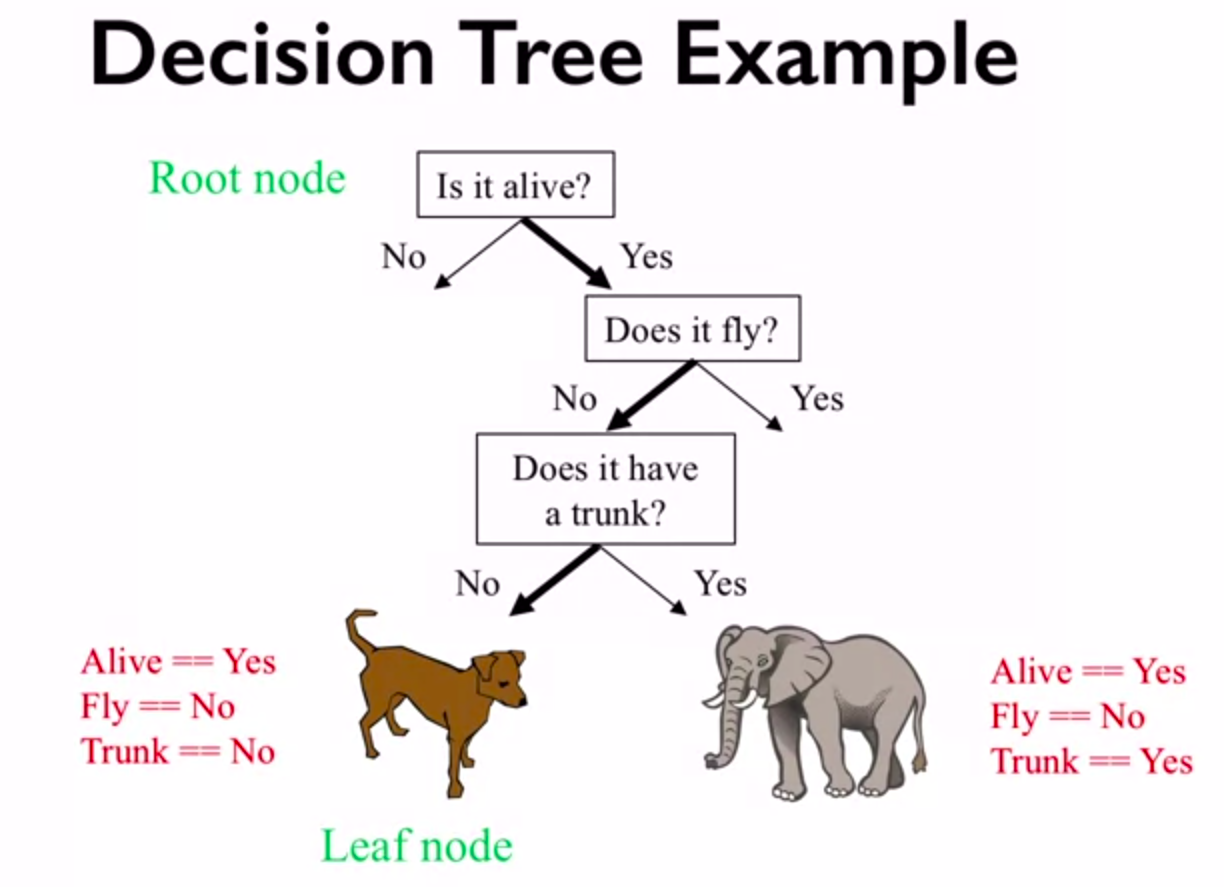
\includegraphics[width=8cm]{"images/dTreeExample.png"}
  %\centering
\caption*{Fonte: }%%"https://machine-learning-and-data-science-with-python.readthedocs.io/en/latest/assignment5_sup_ml.html"}
  \label{dTree}
\end{figure} 

O exemplo na figura \ref{dTree}, ilustra uma árvore de dicisão utilizada para decidir com base em caractetísticas dadas, se o objeto estudado é um elefante. O processo começa olhando para todo o banco de dados e perguntando se é um ser vivo ou não. Caso negativo, ja é suficiente para afirmar que não é um elefante. No caso positivo, são feitas outras perguntas a fim de se ter mais certeza da respósta final. Desta forma a cada divisão temos subgrupos para os quais vamos tomando decisões ou fazendo novas perguntas até que se chegue numa decisão.


Cada divisão feita pela árvore é chamada de partição, ou ramo, enquanto cada subamostra gerada é chamada de nó. O primeiro nó, também conhecido como Nó inicial contém todo o banco de dados, os nós seguintes são chamados de nós intermediários enquanto os nós que não tem nenhuma divisão posterior, ou seja, os nós em que temos uma decisão, são chamados de nó folha ou nó final. 

Para partiçaõ dos nós, ocorrem divisões binárias baseadas  em medidas de impureza (Entropia, Gini, etc.), tais divisões, tem o objetivo de trazer subamostras cada vez mais parecidas em relação a variável que está sendo classificada. No entanto estas divisões podem ocorrer de forma extensa, trazendo árvores grandes e provocando \emph{ovefitting}, uma forma de limitar isso é criando algum critério de parada para a árvore. Diferentes critérios de parada podem ser utilizados de acordo com o objetivo e o problema abordado.



\subsubsection{Bagging}

O Bagging(Boootstrap Aggregation) é um classificador Ensemble.

Os classificadores do tipo Ensamble tem o objetivo de trazer melhores predições através do ajuste de multiplos modelos e a combinação de seus resultados. 

A ideia de combinar modelos serve para contornar limitações que podem vir de um modelo ajustado sozinho. No contexto de Ensamble, os modelos sozinhos são chamados de week learners ou modelos basicos. E estes modelos básicos que poderiam não performar muito bem sozinhos, são utilizados como base para a construção de modelos mais complexos com menor variância e/ou vicio do que cada modelo individual.

Após pensar em combinar modelos, o próximo passo é pensar em como fazer essa combinação. Uma das formas de combinar estes modelos é através do método conhecido como bagging. 

A ideia do bagging é ajustar modelos basicos que não dependam um do outro e depois combinar suas decisões.

Os modelos são ajustados de forma independente e por diferentes conjuntos de dados. os diferentes conjuntos de dados são definidos através da técnica de reamostragem bootstrap, que busca uma nova amostra a partir da extração com reposição dos valores da amostra inicial.

Após os diferentes modelos ajustados com as diferentes amostras, o resultado final será o resultado médio dos modelos. Nos casos de classifição, o valor mais frequente. Por exemplo, se treinassemos um modelo para prever se iria ou não chover no próximo dia, ao utilizar o bagging com 10 modelos, se 6 deles indicassem chuva, e 4 deles indicassem que não choveria, o resultado final seria o indicativo de chuva.


\subsubsection{Floresta Aleatória}


Por fim, chegamos nas Florestas aleatórias que são modelos bagging que usam árvores de decisão como modelos basicos.

Dizendo de modo simples, o algoritmo de florestas aleatórias cria várias árvores de decisão e as combina para obter uma predição.

O uso de florestas aleatórias ajuda a evitar alguns problemas que seriam observados nas árvores sozinhas, uma das maiores vantagens é que as  florestas dificultam a ocorrência de overfitting. Por outro lado, uma das desvantagens é que devido ao ajuste de multiplos modelos, o algoritmo pode ficar lento e dificultar a predição em tempo real.

%%%%%%%%%%%
\subsection{SVM - Suport Verctor Machine}
O objetivo das maquinas de vetores de suporte é encontrar um hipeplano em um espaço n-dimensional que consiga separar os pontos de categorias distintas. Um exemplo visual da separação de duas categorias utilizando  hiperplanos é mostrado na figura \ref{fig: hiperplanes}

\begin{figure}[ht]
\centering
\caption{Hiperplanos nos espaços 2D e 3D}
  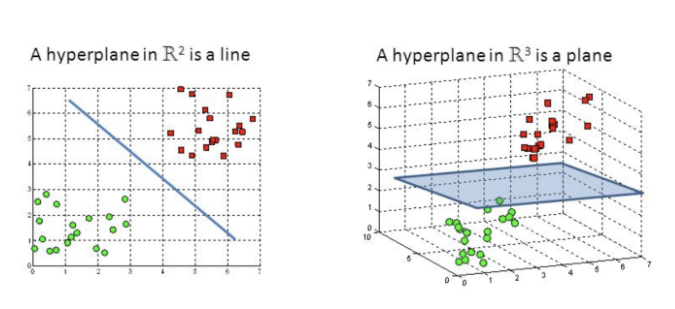
\includegraphics[width=8cm]{"images/hiperplaneExample.png"}
  \centering
\caption*{Fonte: }%%"https://towardsdatascience.com/support-vector-machine-introduction-to-machine-learning-algorithms-934a444fca47"
\label{fig: hiperplanes}
\end{figure} 

No caso de SVM, que são classificadores binários, é usual utilizar  -1 e 1 para especificar as respóstas, tendo então um classificador da segunte forma:

se $f(x) = \beta_0 + \beta_1x_1 + ... + \beta_px_p  < 0$ então Y = -1


se $f(x) = \beta_0 + \beta_1x_1 + ... + \beta_px_p  > 0$ então Y = 1

Na figura \ref{fig: hiperplanes} temos o exemplo de apenas um hiperplano separando cada cenário, mas é fácil ver que poderiam haver outros fazendo tal separação. No caso de haver masi de um hiperplano capaz de separar, o hiperplano ideal será o que maximiza a distância entre entre os pontos das duas classes. Esta distância é chamada de margem.

As margens são definidas pelos pontos mais próximos do hiperplano, estes pontos são os chamados vetores de suporte, pontanto a margem é definida pela distância entre vetores de suporte de classes diferentes. Um exemplo visual é mostrado na figura \ref{fig: marginsSuportVerctorExample}.

\begin{figure}[ht]
\centering
\caption{Exemplo de margem e vetores de suporte}
  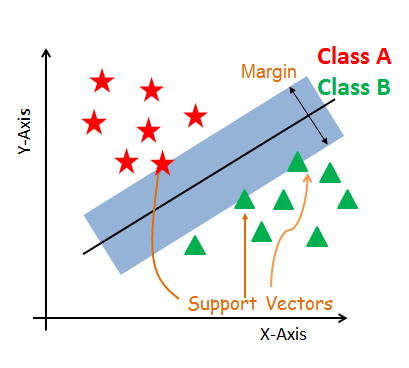
\includegraphics[width=6cm]{"images/marginsSuportVerctorExample.png"}
  \centering
\caption*{Fonte: }%%"https://www.datacamp.com/community/tutorials/svm-classification-scikit-learn-python"
\label{fig: marginsSuportVerctorExample}
\end{figure}

Todos os exemplos mostrados até agora apresentam um cenário ideial, onde um hiperplano separa de forma linear as duas classes, no entanto é comum que não haja um hiperplano que separe as duas classes perfeitamente. Uma solução para isso é permitir que alguns pontos sejam classificados erroneamente, essa abordagem torna o algoritimomenos sensível á pequenas mudanças nos dados e pode aumentar seu poder preditivo.

Outra forma de abordar o problema é obtendo separações mais complexas que hiperplanos, para isso podemos fazer transformações nas variáveis e utilizar svm nessas novas variáveis transofrmadas. No entanto essa transformação pode aumentar o número de variáveis na base e tornar os calculos mais complexos e pesados computacionalmente. Uma forma de abordar esse problema é utilziando o truque de Kernel quando queremos aplicar transformações em variáveis.

Essencialmente, a ideia do truque de Kernel é tranformar as variáveis em uma forma mais geral e computacionalemnte atrativa, utilizando somente produtos internos entre todas as observaões para calcular os coeficientes, ao invés de precisar calcular todas as variáveis tranformadas. Utilizando este truque, o produto interno das variáveis transformadas poderá ser escrito através de uma função(kernel) do produto interno das variáveis originais, fazendo com que seja possível encontrar os coeficientes de uma tranformação, sem de fato a fazer.

Quando utilizamos o truque de kernel, usualmente, pensamos no kernel que pode se aplicar ao invés de pensar primeiro na rtansofmrçaõ para depois verificar se pode ser utilizado o truque.

Um dos kernels mais conhecidos é o kernel polinomial de grau d : $K(x_i,X_j) = (1 + <x_i,x_j>)^d$. Em cada problema diferentes kernels terão desempenhos melhores ou piores.

O calculo dos hiperplanos utilizando um kernel terá o efeito de ter uma tranformação feita sem de fato a fazê-la.


%%%%%%%%%%%
\subsection{Análise discriminate}


%%%%%%%%%%%
\subsection{Avaliação de modelos de classificação}

%%%%%%%%%%%
%\subsection{Avaliação de modelos de tempo **** Melhorar esse nome}
   


%%%%%%%%%%%%%%%%%%%%%%%%%%%%%%%%%%%%%%%%%%%%%%%%%%%%%%%%%%%%%%%%%%%%%%%
%%%%%%%%%%%%%%%%%%%%%%%%%%%%%%%%%%%%%%%%%%%%%%%%%%%%%%%%%%%%%%%%%%%%%%%
%%%%%%%%%%%%% Simulação dos dados
\section{Simulação e tratamento dos dados} % criando seção dentro do capítulo
Para a criação de modelos de collection score, são considerados dados referentes á diversos aspéctos relacionados ao perfil do cliente e ao seu comportamento e relacionamento com a instituição. No entanto estes dados são de difícil acesso, as empresas que detem este tipo de dado não os disponibilizam, tanto por questões de privacidade dos dados de seus clientes quanto por questões estratégicas.

Para desenvolver os modelos deste trabalho, utilizamos dados simulados. A simulação foi feita pensando em uma base de inadimplência de IPTU. E de acordo com estudos e experiências referentes ao mercado de crédito e inadimplência levantamos as seguintes variáveis para serem simuladas:

\begin{itemize}

 \item \textbf{Proprietário}: Indicador se o devedor é dono do imóvel. (0,1)
 \item \textbf{Tempo de relacionamento}: Tempo em meses que devedor tem relação com o imóvel em questão.(0 a 60)
 \item \textbf{Idade}
 \item \textbf{Proprietário}: Idade do devedor, limitada entre 18 e 60 anos
 \item \textbf{Score Serasa}: Score Serasa do devedor. (0, 1000)
 \item \textbf{Quitação}: Tipo de quitação da dívida (Integral, Parcelado, Parcelado com Dívida ativa)
 \item \textbf{Pagamento}: Indicados se ja houve pagamento de parte da dívida (Parcial, Sem pagamento)
 \item \textbf{Natureza da Dívidade}: Indicador se a dívida ocorreu devido a alguma fraude (Devedor, Fraude)
 \item \textbf{Atraso anterior}: Indicador se houve algum atraso anterior de alguma outra dívida. (Sim, Não)
 \item \textbf{Responsabilidade solidária}: Indicador das responsabilidades do imóvel estarem sob o devedor ou se houve algum tipo de responsabilidade conjunta ( Sim e Não)
 \item \textbf{Protestos}: Quantidade de protestos atribuidos ao cliente ( 0,1, ..)
 \item \textbf{Dívidas executadas}: Quantidade de dívidas cobradas na justiça (0,1, ...)
 \item \textbf{Dívidas ativas}: Quantidade de dívidas ativas (0,1,...)
  \item \textbf{Garantias e Penhores}: Indicados de comprometimento do cliente com alguma garantia ou penhor. ( Sim, Não)
  \item \textbf{Prescrição}: Indicador de haver dividas anteriores que foram prescritas. ( Sim, Não)
  \item \textbf{Proprietário, restituição ou indenização}: Indicador se há algum precatário, restituição ou indenização a ser recebida pelo devedor.
  \item \textbf{negociaçãoanteior} Indicador de negociações anteriores para evitar dívidas.  (Sim, Não)
  \item \textbf{regularidadeAcessorias} Indicador de falta de regularidade relacionadas as atividades econômicas de empresas das quais a pessoa é dona ou sócia. (Sim, Não)
  \item \textbf{Saldo devedor}: percentual do total da dívida a ser quitado.(0 a 1)
     
\end{itemize}

A simulação de cada variável foi feita de forma aleatória uniforme, com exeção das variáveis que indicavam quantidade de protestos e dívidas, que foram simuladas a partir da distribuição Poisson com média 1.

Após a simulação das variáveis individualmente, foi feito o agrupamento delas em um data frame, neste ponto, as variáveis numéricas foram padronizadas para obedecerem a mesma escala. A escolha da padronização das variáveis numéricas foi feita pelo fato de que usualmente durante o ajuste dos modelos, as variáveis são padronizadas, então a padronização foi feita nesta etapa.

Outro ponto abordado foi o encoding das variáveis categóricas, as variáveis dicotômicas foram tranformadas em uma coluna binárias, e as variáveis com mais de uma categoria foram espandidas em uma coluna dicotômica para cada categoria.

Para simular se a dívida teve pelo menos 80\% de seu valor pago, utilizamos a função logística para estimar as probabilidades do valor ser pago. Os valores de beta são pesos que foram definidos com base em conhecimentos anteriores e estudos sobre o assunto para definir o impacto de cada variável no pagamento da dívida. Tendo calculado as probabilidades, utilizamos a função rbinom do software R, para simular os dados ponderando com as probabilidades calculadas.

A distribuição da variável resposta simulada é mostrada a seguir:



 \begin{center}
 \textbf{Inserir aqui o gráfico}
\end{center}


O próximo ponto de interesse é simular o tempo nescesário para que a dívida seja paga. Para isso, foi feita a simulação para dados de sobrevivência, a partir das observações que foram definidas que pagariam parte da dívida. O período de tempo estipulado foi de 180 dias, portanto, simulamos a partir da função sim.survdata do pacote coxed do software R o tempo nescessário para que a dívida fosse paga em pelo menos 80\% de seu total. 

A consideração foi a mesma para os pagamentos parcelados ou integrais, nos integrais, é considerado o tempo para o pagamento total e no parcelado é considerado o tempo em que é paga a parcela que atinge 80\% do valor da dívida.

A distribuição do tempo simulado para pagamento é mostrada a seguir:

\begin{center}
 \textbf{Inserir aqui o gráfico}
\end{center}


Tendo sido feitas as simulações do banco de dados, foi iniciado o processo de ajuste e comparação de modelos.
%\cite{rstudio}


%\bibliography{teste}


\end{document}



















%%%%%%%%%%%%%%%%%%% COisas que posso precisar no documento


%% PAra não identar alguma coisa:
%%\noindent
